\documentclass[11pt]{article}

\usepackage{amsmath}
\usepackage{graphicx}
\usepackage{multicol}
\usepackage{wrapfig}
\usepackage{hyperref}
\usepackage{tabularx}
\usepackage{setspace}
\usepackage{comment}
\usepackage{color}

\usepackage[compact]{titlesec}  
\titlespacing{\section}{0pt}{0pt}{0pt}
\titlespacing{\subsection}{0pt}{0pt}{-5pt}
\titlespacing{\subsubsection}{0pt}{0pt}{-5pt}

\oddsidemargin 0cm
\evensidemargin 0cm

\usepackage[margin=1in]{geometry}

\parindent 0cm
\parskip 0.5cm

\usepackage{fancyhdr}
\pagestyle{plain}
%\fancyhf{}
%\fancyhead[L]{AOSS Reference Sheet}
%\fancyhead[CH]{test}
\fancyfoot[C]{Page \thepage}

\newcommand{\vb}{\mathbf}
\newcommand{\diff}[2]{\frac{d #1}{d #2}}
\newcommand{\diffsq}[2]{\frac{d^2 #1}{{d #2}^2}}
\newcommand{\pdiff}[2]{\frac{\partial #1}{\partial #2}}
\newcommand{\pdiffsq}[2]{\frac{\partial^2 #1}{{\partial #2}^2}}
\newcommand{\topic}{\textbf}
\newcommand{\arcsinh}{\mathrm{arcsinh}}
\newcommand{\arccosh}{\mathrm{arccosh}}
\newcommand{\arctanh}{\mathrm{arctanh}}

\begin{document}

\appendix

\addtocounter{section}{3}
 
\section{Project Description}

%The National Research Council has also acknowledged that ``climate models are continually moving toward higher resolutions via a number of different methods in order to provide improved simulations and more detailed spatial information'' \cite{NRC2012CLIMATEMODELS}.  

The next century is expected to see unprecedented changes to the climate system with extensive socioeconomic repercussions.  Since large-scale intervention and experimentation on the Earth system is impossible, global atmospheric modeling systems have been built to provide a laboratory for understanding future climate change.  Although these models have led to a strong consensus on the global-scale changes that will occur over the next century, many outstanding questions remain on how regional or local climate will be affected.  In particular, understanding extreme temperatures, precipitation and weather events is key for informing local policymakers and communities, and developing adaptation policies.  However, restrictions on computational cost have inherently limited the finest resolution of our uniform-resolution global atmospheric models to 50-100 kilometers, far beyond the scale necessary for capturing many facets of regional climate.  Dynamically downscaled simulations that use global climate model data for driving the boundary conditions of regional-scale models are also known to suffer from spurious boundary noise due to inconsistencies in the regional and global numerics.  Consequently, there is a pressing need to develop a next generation of global atmospheric modeling systems that can reach high spatial resolutions and local scales.

In response to the aforementioned need, the goal of this proposal is to develop, analyze and implement new numerical methods for a next-generation atmospheric modeling system that
\vspace{-0.4cm}
\begin{enumerate}
\item[(a)] provides the \textbf{most accurate solution of the equations of motion} while limiting the need for artificial numerical diffusion,
\item[(b)] is scalable (in both a strong and weak sense) on \textbf{massively parallel computers},
\item[(c)] is valid on resolutions finer than 10km by solving the \textbf{non-hydrostatic global equations},
\item[(d)] addresses \textbf{known numerical issues with existing terrain-following coordinate models} at high horizontal resolutions, including horizontal pressure gradient errors, and
\item[(e)] supports \textbf{static and adaptive mesh refinement} to address questions on regional and local scales and improve representation of weather extremes.
\end{enumerate}

\vspace{-0.4cm}
The focus of this proposal will be \textbf{staggered nodal finite element methods (SNFEMs)}, which can be thought of as an optimal mixture of continuous and discontinuous nodal finite element methods (NFEMs).  These methods are described in detail in section \ref{sec:SNFEM}.  The central hypotheses of this proposal are as follows:

\vspace{-0.4cm}
\begin{itemize}
\item[(H1)] Horizontally staggered nodal finite element methods will provide an optimal or near-optimal treatment of wave-like features, energy and enstrophy conservation and will reduce the need for significant artificial numerical diffusion / stabilization compared to unstaggered methods.

\item[(H2)] Vertically staggered nodal finite element methods will improve the ability of the model to capture vertical stratification in the atmosphere, and improve the treatment of the pressure gradient force near rough topography.

\item[(H3)] A non-linear numerical diffusion operator based on either a variational multi-scale (VMS) or upwinding can be used to reduce diffusive errors in the finite element formulation over hyperviscosity, especially in the presence of steep topography gradients.
\end{itemize}

These hypotheses and proposal goals will be addressed via a structured set of research tasks:

\vspace{-0.4cm}
\begin{itemize}
\item[(T1)] \textbf{Analyze the wave-like behavior} of the 1D and 2D SNFEMs and NFEMs under modified order-of-accuracy, prognostic variable staggering and choice of flux reconstruction function.

\item[(T2)] Implement 1D SNFEMs for \textbf{discretization of the vertical coordinate} in the Tempest framework.  Analyze and contrast model results using the vertical SNFEM formulation.  Test sensitivity of horizontal pressure gradient errors to vertical order-of-accuracy and staggering.

\item[(T3)] Implement 1D SNFEMs for \textbf{discretization of the horizontal coordinate} in the Tempest framework.  Analyze and contrast model results for different choices of staggering, order-of-accuracy and viscous coefficients.

\item[(T4)] Develop and implement variational multi-scale (VMS) and upwind-type \textbf{dissipation mechanisms for both horizontal and vertical finite element discretizations}.  Analyze and compare simulation results.

\item[(T5)] Extend the Tempest framework to support \textbf{static and adaptive mesh refinement} with SNFEMs.
\end{itemize}

\vspace{-0.4cm}
The focus of this proposal on the development, analysis and implementation of new numerical methods fits well within the scope of NSF Computational Mathematics, which supports ``mathematical research in areas of science where computation plays a central and essential role, emphasizing design, analysis, and implementation of numerical methods and algorithms, and symbolic methods.''  A further strength of this proposal is its interdisciplinary character, bridging atmospheric science (represented by PI Ullrich) and computational mathematics (represented by co-PI Persson).  The numerical methods developed under this project will further have interdisciplinary application, and will be useful to disciplines such as acoustics, aerospace, astrophysics and oceanography.

The remainder of this proposal is as follows:  Broader impacts and intellectual merit are described in section \ref{sec:BroaderImpacts}.  The background, motivation and problem statement is provided in section \ref{sec:BackgroundMotivation}, followed by the proposed strategy in section \ref{sec:ProposedStrategy}.  The detailed research tasks  is found in section \ref{sec:Research} and the research plan and timeline in section \ref{sec:ResearchPlan}.

\subsection{Broader Impacts and Intellectual Merit} \label{sec:BroaderImpacts}

This proposal tackles the development of new numerical methods that improve the efficiency and accuracy of global climate and weather forecasting systems.  The methods discussed in this proposal will have direct societal implications:
\vspace{-0.4cm}
\begin{itemize}
\item High-resolution and multi-resolution methods are directly applicable to regional scale climate problems: Changes in the behavior of mesoscale storm systems, pressure blocking events driven by topography (responsible for heat waves and cold spells), mountain snowpack, wildfires, topographically-driven precipitation, watershed-level hydrology, urban development and agriculture are all regional scale issues that are poorly addressed in current generation global climate modeling systems.
\item Regions of sharply varying topography, such as at the periphery of the California central valley or the Rocky Mountains, will be better represented by global models.
\item The improved treatment of wave-like motion by these methods will provide enhancement of atmospheric features, such as the Madden-Julian Oscillation (MJO).
\item The multi-resolution framework produced in this proposal can be used to test sub-grid-scale physics at a fraction of the cost of global high-resolution models.
\end{itemize}
\vspace{-0.4cm}
This project seeks to improve the partnership between computational scientists and atmospheric scientists by a mutual exchange of expertise on computational fluid dynamics.  The modeling tools built as a consequence of this proposal will provide a much-needed update to existing technologies.  All products will be released as open source in both standalone form and as a dynamical core option in the Community Earth System Model (CESM) \cite{JWHetal2013BAMS}.  The code for this project will be released under the Lesser GNU Public License (LGPL),which allows largely unrestricted access to the technology developed as part of this effort.  This project is further aimed at funding the thesis work of a graduate student through completion of their degree.

This project will further tie into the Dynamical Core Model Intercomparison Project (DCMIP), a major international effort that focuses on assessment of computational methods for solving the atmospheric fluid equations \cite{DCMIP2012TESTCASES,kent2013dynamical}.  The PI is currently a lead organizer of this effort.  DCMIP has previously run a two-week summer school and workshop in the summer of 2008 and 2012, with the next workshop planned for June 2016.  These workshops have historically attracted over a dozen international modeling groups and over 30 graduate students for an intensive educational experience for participants in global modeling.  The next workshop will specifically focus on developing numerical methods for simulating at high resolution, multi-resolution modeling and the coupling of model dynamics and physics.  It is expected that the graduate student and postdoc funded as part of this proposal will represent and showcase this work at the DCMIP workshop.

\subsection{Background and Motivation} \label{sec:BackgroundMotivation}

\subsubsection{The need for an accurate treatment of wave-like motion} \label{sec:AccurateWaves}

To a close approximation, the global atmosphere is in a state of geostrophic and hydrostatic balance.  The dynamic character of the atmosphere is governed by a slow adjustment process that gives rise to wave motion over all scales.  \textbf{Accurate treatment of wave-like motion is of paramount importance to capturing departures from balance, and to ensure that the adjustment process is correct and free from spurious numerical errors} \cite{randall1994geostrophic, thuburn2005vertical}.

In atmospheric models there is a need for even the shortest resolved waves to be treated accurately.  Since many important atmospheric features are largely unresolved at even the finest global model resolutions, dynamical models are dependent on sub-grid-scale \textit{parameterizations} for representing features such as turbulence, convection and moist processes.  These parameterizations apply a forcing to the dynamics all the way down to the grid scale.  To ensure a correct dynamical response to grid-scale forcing, the discretization must be able to accurate capture wave-like behavior at the shortest resolved wavelengths.

%Sound waves are the fastest moving waves in the atmosphere (330 m/s), but are largely irrelevant for modeling large-scale weather patterns, whereas bulk atmospheric waves (Rossby waves and inertia-gravity waves) only reach speeds of at most 100 m/s in the upper tropospheric jets.  

The need for an accurate treatment of waves in atmospheric models led to global spectral models (which perfectly capture linear dispersion relationships) being the dominant discretization for over three decades \cite{bourke1972efficient, gordon1982description, barros1995ifs}.  These models have only recently fallen out of favor as a consequence of their poor scalability on large-scale parallel systems (discussed further in section \ref{sec:FEM}).  The need for parallel scalability is a growing need:  Atmospheric simulations are a benchmark application for exascale computing systems since many important climatological features are unresolved at current resolutions.  Consequently, any improvement to the simulation quality has the potential to significantly reduce computational expense by improving simulations quality at coarser resolutions.

\subsubsection{The need for non-hydrostatic models} \label{sec:UniqueAtmosphere}

The atmosphere has many other unique features which must be accounted for in any model.  First, the atmosphere itself only occupies a thin shell around the Earth of approximately $100\ \mbox{km}$ thickness, relative to the Earth's circumference of $40,030\ \mbox{km}$.  Second, although the atmosphere is largely uniform horizontally, it is strongly stratified in the vertical, with pressures of $10^5\ \mbox{Pa}$ at the Earth's surface to $100\ \mbox{Pa}$ at the top of the stratosphere.  Third, the bottom of the domain is a rough unresolved boundary with local steepness that is strongly dependent on model resolution.

In global atmospheric models, the domain is typically discretized at a horizontal resolution of approximately $110\ \mbox{km}$ and a vertical resolution ranging from $100\ \mbox{m}$ in the lowest model levels to $3-4\ \mbox{km}$ near the model top.  The highest resolution uniform models that have been used for climate experiments are only at scales of $25\ \mbox{km}$, due to constraints on available computing power.  Variable-resolution modeling systems, which are capable of providing enhanced resolution over a particular regional patch, have recently been a subject of substantial interest and have pushed local climate resolution down to $10\ \mbox{km}$.  Nonetheless, even at these (relatively fine) horizontal resolutions, the horizontal-vertical aspect ratio is on the order of $\sim 100$.  Consequently, in accordance with the Courant-Friedrichs-Lewy (CFL) condition, the use of explicit time stepping in the vertical would greatly restrict the maximum time-step size.  To overcome this difficulty, the hydrostatic approximation has traditionally been used to enforce instantaneous balance between the vertical pressure gradient force and gravity and so eliminates vertically propagating sound waves.  However, this approximation ignores horizontal transport of vertical velocity and so is no longer valid for horizontal grid resolutions below approximately $10\ \mbox{km}$.

With horizontal resolutions quickly approaching this limit, \textbf{the next generation of modeling systems will need to adopt the Navi\'er-Stokes equations in their unapproximated form} (an area of ongoing research, and the focus of this proposal).  Models using these equations are typically referred to as \textbf{non-hydrostatic models}.  To avoid the vertical CFL limitation, these systems have generally adopted an explicit temporal discretization in the horizontal in conjunction with an implicit temporal discretization in the vertical, also known as Horizontally Explicit Vertically Implicit (HEVI), coupled in the context of an Implicit-Explicit Runge-Kutta (IMEX-RK) framework \cite{UASJRRJS1997AMM, PAUCJ2012MWR, HWSJLNW2013JCP}.

%Fourth, unresolved physical processes on the sub-grid-scale, including condensation, vertical convection, turbulence and radiation, lead to forcing of the resolved-scale flow at the finest grid scales.

\subsubsection{Topography and the pressure gradient problem} \label{sec:TopographyPGF}

Model topography is typically introduced by transforming the vertical coordinate so that the Earth's surface becomes a coordinate surface \cite{TGCRCJS1975JCP, schar2002new}.  Compared with alternatives, such as cut cells \cite{causon2000calculation, ingram2003developments}, immersed boundary methods \cite{mittal2005immersed} or embedded boundary methods \cite{johansen1998cartesian, wang2011algorithms}, this approach is simple and is easily implemented with high-order accuracy.  However, this approach also has one key disadvantage:  a straightforward implementation of terrain-following coordinates leads to coordinate surfaces which are not aligned with ``surfaces of constant stratification.''  This in turn can lead to two types of errors in atmospheric models:  First, since pressure and density gradients in the vertical are much stronger than their counterparts along constant height surfaces, computed horizontal pressure gradients (which are computed along terrain-following surfaces and then corrected) are polluted by the effects of vertical stratification.  Second, stabilization of horizontal dynamics often uses viscosity operators \cite{dennis2011cam} that ignore stratification completely, which in turns leads to an unphysical diffusion of density and pressure along coordinate surfaces.  Both of these errors are responsible for driving the atmosphere away from hydrostatic balance, and leading to the generation of unphysical horizontal and vertical velocities.

These errors are most pronounced near regions with the strongest topographic gradients.  Figure \ref{fig:OmegaNoise} shows the one-year average upper-tropospheric vertical pressure velocity ($dp/dt$) field above the Himalayas with the spectral element dynamical core of CESM.  Readily apparent and spurious numerical noise arises due to a poor treatment of pressure gradients in terrain-following coordinates that is only remedied by greatly smoothing out the underlying topography (and reducing the effective resolution of the model).  At higher horizontal resolutions, this problem is only expected to worsen:  Since the sharpest gradients in topography are typically adjacent to local peaks, an increase in horizontal resolution is expected to lead to steeper slopes.  A simple example of this problem is depicted in Figure \ref{fig:MountainSlopeResolution}, where an isolated Utah mountain is plotted with a variable horizontal resolution.  As the horizontal mesh is refined, the maximum slope also increases in steepness to $32^\circ$ at the finest resolution.

%This problem has significant implications for global atmospheric modeling, with efforts to tackle this problem stretching back as far as the late 1970s \cite{ZIJ1977BzPdA, DTMZIJ1986MAP}.  The typical solution to this problem is to apply a diffusive filter to topography data until the maximum slope fits within a specified tolerance and there is no sign of numerical noise associated with steep topography.  This approach has the obvious consequence of severely damaging the quality of the solution near topography, and leading to an effective grid resolution much coarser than the grid would allow.  Topographically driven precipitation, which is particularly important for estimating mountain snow-pack, is weakened substantially under this approach.  Further, atmospheric pressure blocking, which is responsible for stationary pressure systems and the development of heat waves / cold spells, is suppressed under topographical smoothing.

This problem has significant implications for global atmospheric modeling, with efforts to tackle this problem stretching back as far as the late 1970s \cite{ZIJ1977BzPdA, DTMZIJ1986MAP}.  Other approaches that have attempted to address this problem include the use of cut-cells \cite{JSSHPAD2013GMDD}, coordinate surface smoothing \cite{JBK2011MWR}, reconstruction of pressure along horizontal coordinate surfaces \cite{GZ2012MWR}, or formulations which preserve consistency with the continuous operator \cite{SJL1997QJRMS}.  Unfortunately, none of these approaches are considered sufficiently robust, or provide sufficient improvement, to motivate wide acceptance.  Consequently, \textbf{addressing the errors from terrain-following coordinates is one of the major outstanding problems in atmospheric modeling.}

%The pressure gradient problem arises for two reasons:  First, horizontal pressure gradients (which are computed along terrain-following surfaces) can be polluted by the effects of vertical stratification, which in turn drive unphysical horizontal velocities.  Second, current horizontal viscosity operators \cite{dennis2011cam} ignore stratification completely, leading to an unphysical diffusion of density and pressure along coordinate surfaces.  Both types of error can force the equations of motion at the grid-scale and, in conjunction with the stationary wave-modes exhibited by unstaggered schemes, can lead to stationary errors such as those seen in figure \ref{fig:OmegaNoise}.  In the context of high-order FEM, this proposal advocates removing the first type of errors by improving the accuracy of the coupling between the horizontal and vertical discrete pressure gradient operators.  The second type of error will be addressed via the development of a stratification-aware viscous operator.

\begin{figure}[t]
\begin{center}
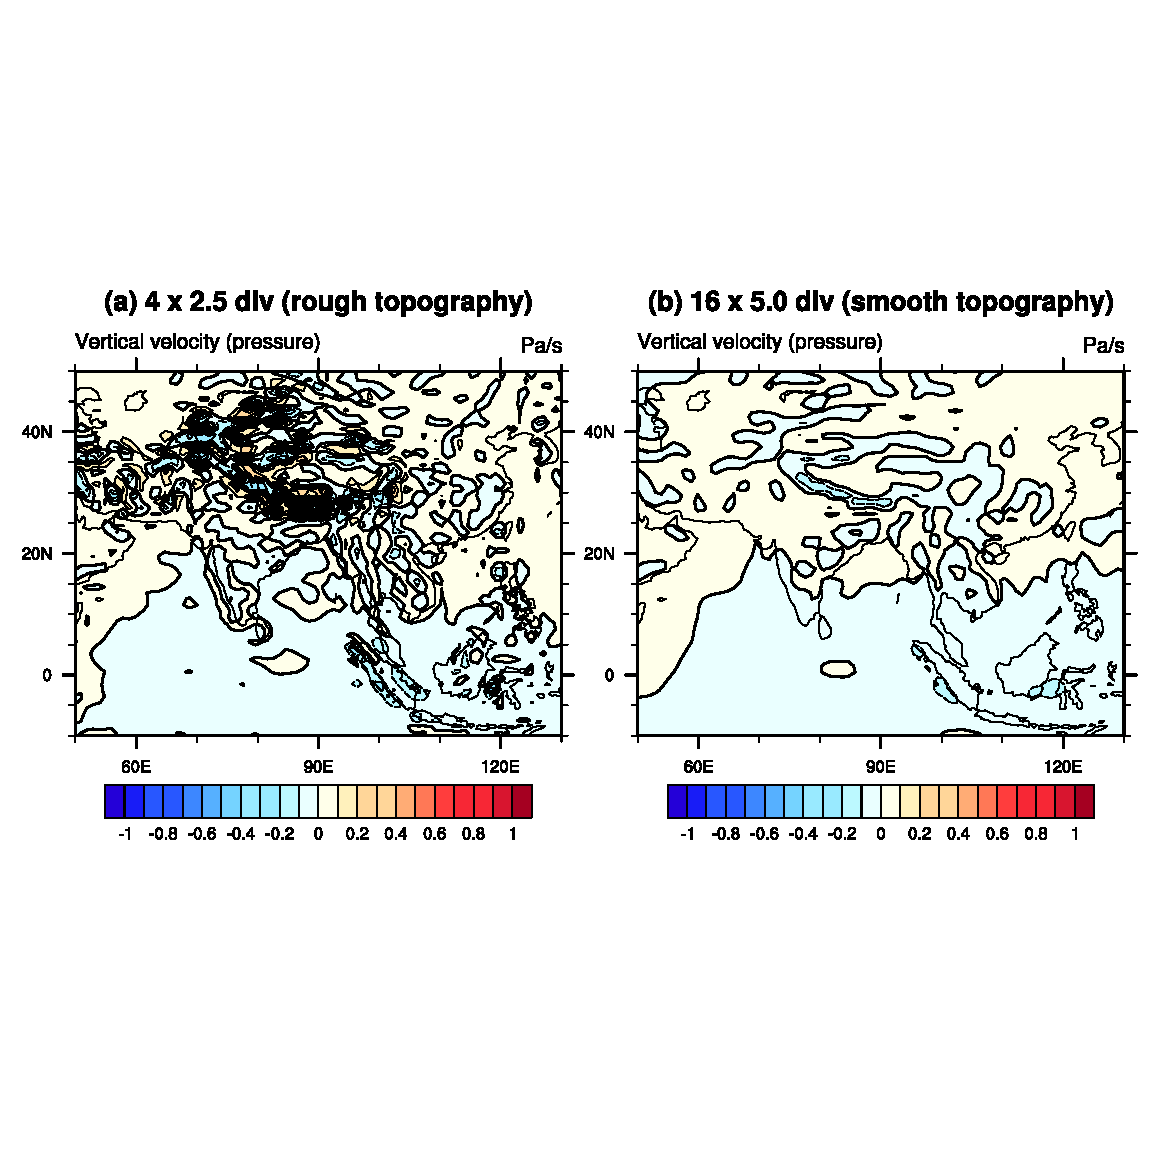
\includegraphics[width=5in, clip=true, trim=0cm 5.1cm 0cm 4.6cm]{OmegaNoise.eps}
\end{center}
\caption{Annual average of $323\ \mbox{hPa}$ (upper tropospheric) vertical pressure velocity over the Himalayas obtained from CESM with (a) a rough topography configuration and (b) a smoothed topography configuration. Because of inaccurate evaluation of the horizontal pressure gradient term, the use of terrain-following coordinates leads to the generation of spurious numerical errors in the presence of steep topography which can produce persistent errors in climate simulations.} \label{fig:OmegaNoise}
\end{figure}

\begin{figure}[t]
\begin{center}
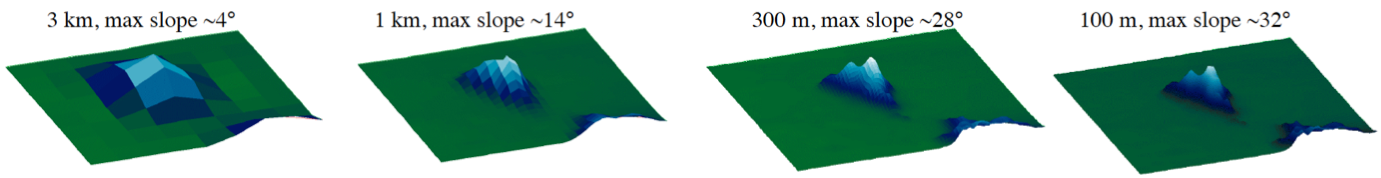
\includegraphics[width=6.5in]{MountainSlopeResolutionLong.png}
\end{center}
\caption{The averaged slope of topography increases monotonically with increased horizontal resolution.  Here an image of an isolated Utah mountain is shown with variable horizontal resolution.  Image courtesy of Dr. Tina Chow, UC Berkeley.} \label{fig:MountainSlopeResolution}
\end{figure}

%{\color{red} [[Pressure gradient figure here]]}

%Under a HEVI discretization, an initially balanced flow over such a mountain will only remain balanced if the pressure gradient terms on the left-hand-side of the horizontal momentum equations (\ref{eq:NonhydroEqn1})-(\ref{eq:NonhydroEqn2}) (those treated via an explicit method) and those on the right-hand-side (treated with an implicit method) cancel each other exactly.  However, a low-order discretization and coupling strategy between the horizontal and vertical discrete pressure gradient terms (that is, standard dimensional splitting) is insufficient to maintain balance.  

%Figure \ref{fig:SpuriousMountainNoise} shows the vertical velocity in the presence of rapidly varying bottom topography, and highlights the effects of inaccurate evaluation of the horizontal pressure gradient term for models with a terrain-following coordinate.  Since typical vertical velocities for large-scale weather systems are $\sim 0.01\ \mbox{m\ s}^{-1}$, these perturbations represent an error of nearly $50\%$.

%The issue of the pressure gradient problem has significant implications for global atmospheric modeling, with efforts to tackle this problem stretching back as far as the late 1970s \cite{ZIJ1977BzPdA, DTMZIJ1986MAP}.  As global models reach to finer spatial scales, the pressure gradient problem leads to an increasingly polluted dynamical solution near steep topography.  The typical solution to this problem is to apply a diffusive filter to topography data until the maximum slope fits within a specified tolerance and there is no sign of numerical noise associated with steep topography.  This approach has the obvious consequence of severely damaging the quality of the solution near topography, and leading to an effective grid resolution much coarser than the grid would allow.  Topographically driven precipitation, which is particularly important for estimating mountain snow-pack, is weakened substantially under this approach.  Further, atmospheric pressure blocking, which is responsible for stationary pressure systems and the development of heat waves / cold spells, is suppressed under topographical smoothing.

%Other approaches which address mitigation of this problem include the use of cut-cells \cite{JSSHPAD2013GMDD}, coordinate surface smoothing \cite{JBK2011MWR}, reconstruction of pressure along horizontal coordinate surfaces \cite{GZ2012MWR}, or formulations which preserve consistency with the continuous operator \cite{SJL1997QJRMS}.


%\begin{figure}
%\begin{center}
%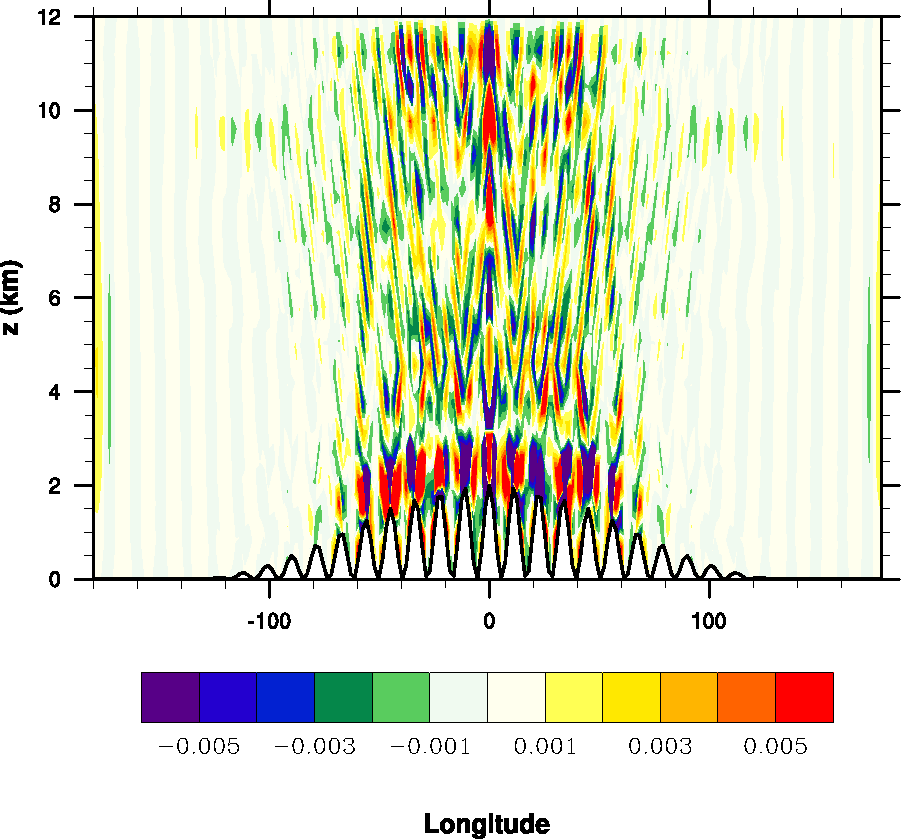
\includegraphics[width=3in]{SpuriousMountainNoise.png}
%\end{center}
%\caption{Vertical velocity for a balanced flow over a rapidly varying mountain range.  Because of inaccurate evaluation of the horizontal pressure gradient term, models with terrain-following coordinates can generate significant spurious numerical errors in the presence of steep topography.  Here a hydrostatically balanced atmosphere initially at rest quickly generates a train of spurious internal mountain waves in response to numerical errors.} \label{fig:SpuriousMountainNoise}
%\end{figure}

%Traditional global atmospheric models use the hydrostatic approximation, which assumes that the vertical atmosphere is perpetually in a state of balance between pressure gradient and buoyancy forces.  In this case, vertical momentum is no longer tracked and is instead diagnosed from other state variables.  However, this approximation breaks down when the horizontal resolution is finer than roughly $10\ \mbox{km}$, and so the next-generation of global atmospheric models have instead turned to using the non-hydrostatic Euler equations (with shallow-atmosphere approximation):
%\begin{align}
%\label{eq:NonhydroEqn1} \pdiff{u^\alpha}{t} + u^i \nabla_i u^\alpha + \frac{1}{\rho} \left[g^{\alpha \alpha} \nabla_\alpha p + g^{\alpha \beta} \nabla_\beta p \right] + f (\vb{k} \times \vb{u})^\alpha &= - \frac{g^{\alpha \xi}}{\rho} \nabla_\xi p, \\
%\label{eq:NonhydroEqn2} \pdiff{u^\beta}{t} + u^i \nabla_i u^\beta + \frac{1}{\rho} \left[g^{\alpha \alpha} \nabla_\alpha p + g^{\alpha \beta} \nabla_\beta p \right]  + f (\vb{k} \times \vb{u})^\beta &=  - \frac{g^{\beta \xi}}{\rho} \nabla_\xi p, \\
%\label{eq:NonhydroEqn3} \pdiff{\theta}{t} + u^\alpha \pdiff{\theta}{\alpha} + u^\beta \pdiff{\theta}{\beta} &= - u^\xi \pdiff{\theta}{\xi}, \\
%\label{eq:NonhydroEqn4} \pdiff{u^\xi}{t} + u^\alpha \nabla_\alpha u^\xi + u^\beta \nabla_\beta u^\xi + u^\xi \nabla_\xi u^\xi &= - \frac{1}{\rho} \nabla^\xi p - g_c, \\
%\label{eq:NonhydroEqn5} \pdiff{\rho}{t} + \frac{1}{J} \pdiff{}{\alpha} (J \rho u^\alpha) + \frac{1}{J} \pdiff{}{\beta} (J \rho u^\beta) &= - \frac{1}{J} \pdiff{}{\xi} (J \rho u^\xi).
%\end{align}  Here $\alpha$ and $\beta$ are arbitrary horizontal coordinates with basis vectors $\vb{i}$ and $\vb{j}$, $\xi$ is a vertical coordinate with unit basis vector $\vb{k}$, the index $i$ spans each coordinate, $g^{ij}$ denotes the contravariant metric, $J = \sqrt{\det g_{ij}}$ is the metric Jacobian, $\nabla_i$ denotes the covariant derivative along the $i^{th}$ coordinate, $g_c$ is gravity, $f$ is the Coriolis parameter, $\rho$ is the density, $\vb{u} = u^\alpha \vb{i} + u^\beta \vb{j} + u^\xi \vb{k}$ is the vector velocity and $\theta$ is the potential temperature.  Einstein summation notation is used for repeated indices.  These equations are closed via the equation of state
%\begin{equation*}
%p = p_0 \left( \frac{R_d (\rho \theta)}{p_0} \right)^{c_p / c_v},
%\end{equation*} where $R_d$ is the ideal gas constant, $p_0$ is a reference pressure and $c_p$ and $c_v$ denote the specific heat capacity of dry air at constant pressure and constant volume.  Observe that (\ref{eq:NonhydroEqn1})-(\ref{eq:NonhydroEqn4}) are given in a non-conservative form; this formulation is generally desirable over the conservative formulation (where momentum and $\rho \theta$ are prognostic variables) since this form can more readily conserve quantities relevant to atmospheric motion, such as angular momentum and potential enstrophy, and (depending on the discretization) can lead to a more accurate treatment of wave-like motions \cite{JTTJW2005JCP}.

\subsection{Proposed Strategy} \label{sec:ProposedStrategy}

\subsubsection{Finite Element Methods and Parallel Scalability} \label{sec:FEM}

The non-hydrostatic equations that govern atmospheric circulation have been known for over a century, and a wide range of mature numerical methods are now available for numerical computation of their solutions.  Finite element methods (FEM), which include both the spectral element (SE) method and the discontinuous Galerkin (DG) method, have a long history in the field of computational fluid dynamics stretching back to the 1970s \cite{patera:84,maday1989spectral,FBSR1997JCP,BCCWS1998JCP,peraire11dg,wang_et_al13cfd}).  Recent advances in FEM \cite{huynh2007flux, ullrich2014global} also no longer impose the need for a conservative equation set when formulated with a DG discretization.  However, FEM have only recently been adopted by the atmospheric modeling community \cite{taylor:97,FXGJSHTW2002JCP,FXGTER2004MWR,AFMTJT2004MWR,NTL2005MWR,FXGMR2008JCP,JFKFXG2012JCP}.  The adoption of FEM in global atmospheric codes is motivated by their near-optimal parallel scalability on large-scale (petascale) parallel systems, and theoretical scalability on future exascale systems, unlike traditional global spectral and semi-Lagrangian methods.   Nodal FEM \cite{hesthaven2007nodal} further exhibit provably minimal bandwidth requirements (that is, they minimize the message size needed to convey information between neighboring elements), a property that can also be incorporated into the discretization of second-order terms using schemes such as the Compact DG (CDG) method \cite{peraire08cdg}.  Figure \ref{fig:CAMSEScalability} shows observed performance of three standard atmospheric dynamics solvers, including the global spectral method (EUL), regular latitude-longitude finite-volume method (FV) and spectral element model (SE).  Only the SE method exhibits near-perfect scalability down to one element per core (86400 cores).  FEM can also be formulated to have many desirable mathematical properties, including mass and energy conservation, high-order accuracy, and discrete preservation of the adjoint and annihilator properties of the gradient, divergence and curl operators.  Further, recent work on FEM has led to techniques for effective positivity and monotonicity filtering \cite{OGMATASC2013}.  Many other modeling groups are now working on adopting finite element methods as the basis for their dynamical cores, including the NUMA model of \cite{JFKFXG2012JCP}.  FEM are also likely candidates for adoption on the U.K. Met Office dynamical core and the upcoming model from the Korean Institute of Atmospheric Prediction Systems (KIAPS).

\begin{figure}[p]
\begin{center}
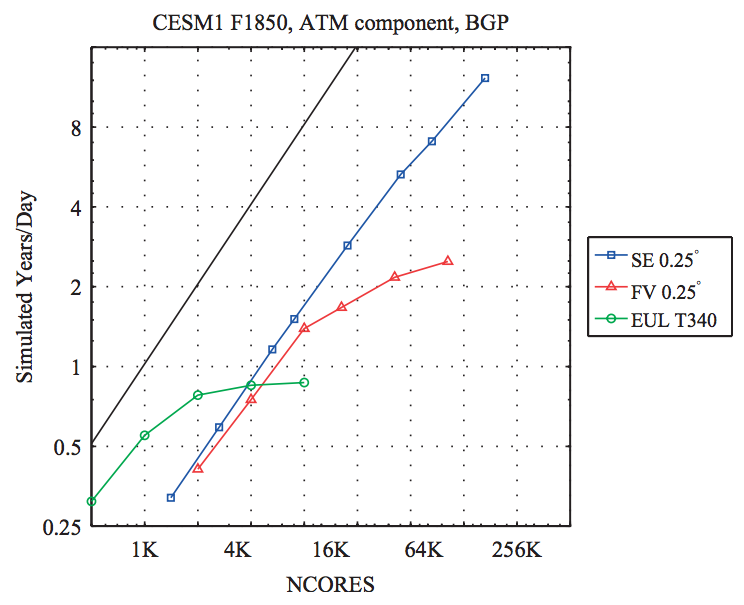
\includegraphics[width=3.5in, clip=true, trim=0cm 1.7cm 0cm 1.7cm]{CAMSEScalability.png}
\end{center}
\caption{Simulated years per day (measuring performance) for three atmospheric dynamical cores at 28km global resolution on Intrepid (IBM BG/P), including the global spectral model (EUL), regular latitude-longitude finite-volume model (FV) and the hydrostatic spectral element model (SE) when run in conjunction with 28km land model and 11km sea ice and data ocean.  Near perfect scalability is observed for the SE model down to one element per core (86400 cores).  Reproduced from \cite{dennis2011cam}.} \label{fig:CAMSEScalability}
\end{figure}

\begin{figure}[p]
\begin{center}
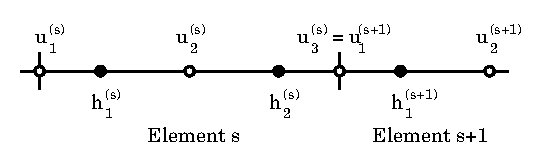
\includegraphics[width=3in]{SEStaggered}
\end{center}
\caption{An example 3rd order horizontal staggering of 1D velocity (u) and height (h) state variables for a continuous/discontinuous SNFEM for the linear wave equation.  Here $u$ nodes are placed at Gauss-Lobatto quadrature points and $h$ nodes are placed at Gaussian quadrature points.  The superscript denotes the element number and the subscript denotes the sub-grid-scale index.} \label{fig:SNFEM}
\end{figure}

\begin{figure}[p]
\begin{center}
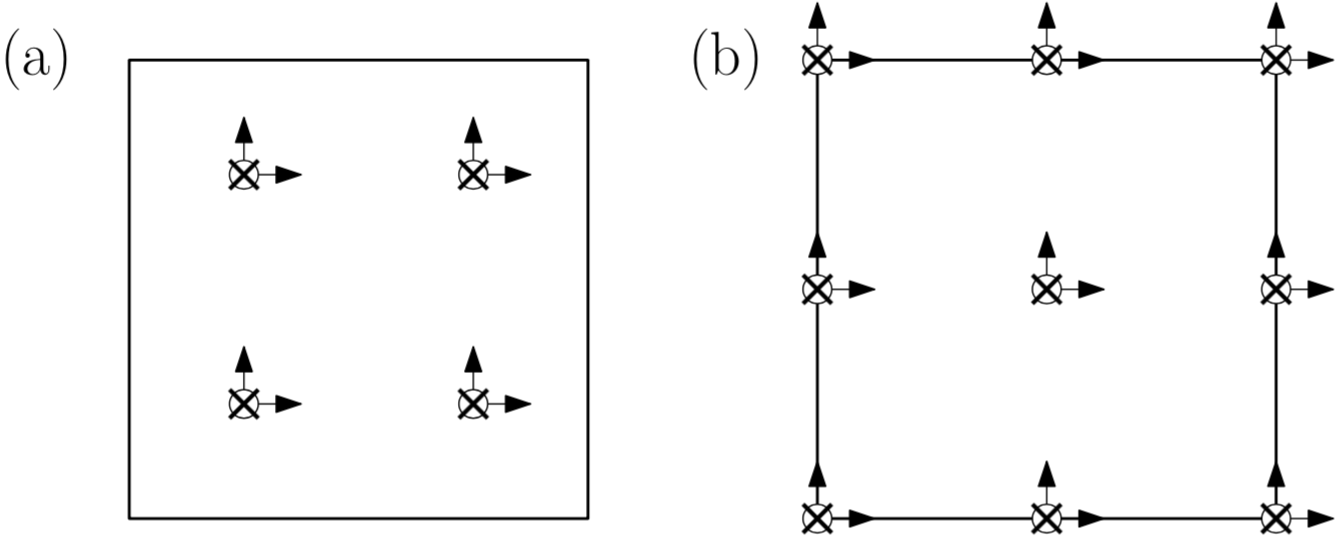
\includegraphics[width=2.5in]{NodalArrangement-Left.png}
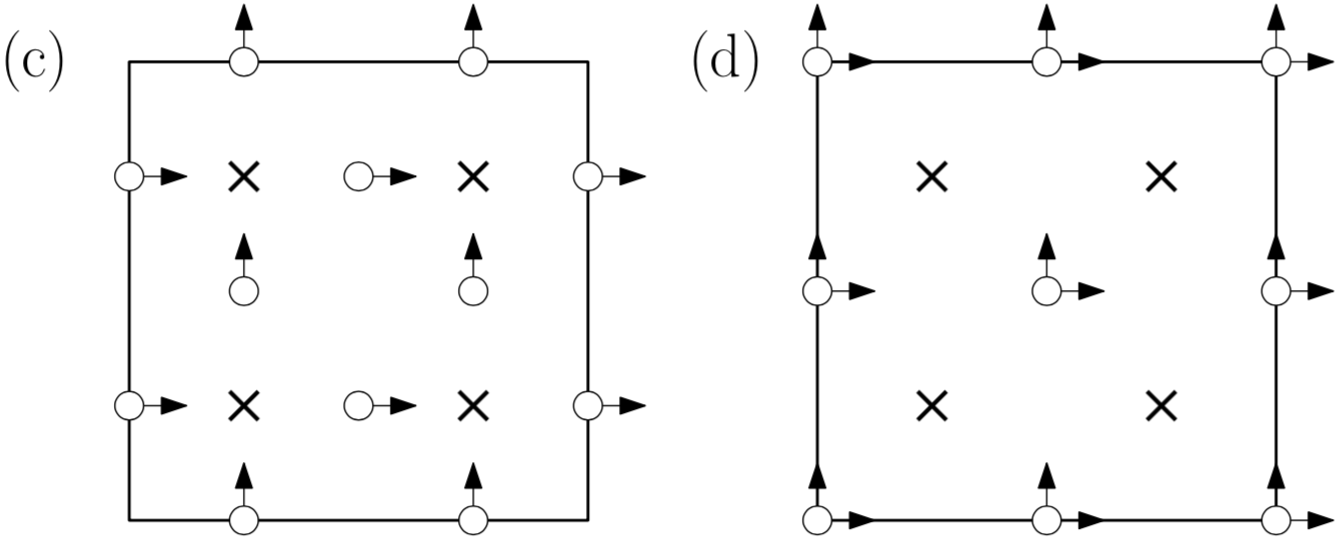
\includegraphics[width=2.5in]{NodalArrangement-Right.png}
\end{center}
\caption{Four options for the placement of scalar ($\times$) and velocity variables (arrows): (a) nodal discontinuous Galerkin, (b) nodal Spectral Element, (c) C-grid SNFEM, (d) B-grid SNFEM..} \label{fig:NodalArrangement}
\end{figure}

\subsubsection{Staggered Nodal Finite Element Methods (SNFEMs)} \label{sec:SNFEM}

Staggered methods, as defined in this proposal, are a class of discretizations where scalar (density, pressure and tracer density) and velocity degrees of freedom are stored at different spatial locations \cite{AAVRL1977GCM}.  These methods have long been used for both horizontal discretizations in atmospheric models \cite{lin2004vertically, putman2009finite, skamarock2005wrf, skamarock2012mpas, thuburn2009numerical} and vertical discretizations \cite{arakawa1988baroclinic, charney1953numerical}.  These methods further have excellent dispersive properties and do not support stationary (zero phase speed) $2 \Delta x$ modes \cite{randall1994geostrophic, thuburn2005vertical, ullrich2014understanding}, which are notorious for polluting atmospheric models.  However, these methods have never been operationally employed above second-order accuracy.  Alongside the rise of finite element methods for atmospheric modeling, there has been a renewed interest in pursuing staggered finite element methods \cite{boffi2009some, cotter2009mixed, cotter2011numerical, cotter2012mixed, staniforth2013analysis} analogous to the mixed-finite element methods employed for elliptic problems \cite{PRJT1977MAFEM}.  Note that this definition of staggering differs from the staggered grid multi-domain method \cite{kopriva1996conservative}, where solution points and flux points are staggered.

This proposal explores \textbf{staggered nodal finite element methods (SNFEMs)}, which are a class of arbitrary order-of-accuracy methods that extend traditional nodal finite element methods (NFEMs) by storing scalar and velocity degrees of freedom at differential spatial locations.  An example nodal staggering for a 3rd order 1D hybrid SE/DG method is depicted in Figure \ref{fig:SNFEM}, where velocity is stored at Gauss-Lobatto (GL) nodes and height is stored at Gauss nodes.  Four possible arrangements of prognostic variables are depicted in Figure \ref{fig:NodalArrangement} for a 2D SNFEM.

Discrete evolution equations for the staggered variables are constructed using an approach that is similar to the flux reconstruction methods of \cite{huynh2007flux}, as described in \cite{ullrich2014global} for non-conservative systems.  Under this formulation, a continuous analogue of the nodal discretization is constructed within an element via polynomial fit through the nodal points associated with a particular variable.  Values and derivatives of the polynomial fits are then evaluated where necessary, augmented (when a discontinuity exists in the reconstruction at element edges) by the derivative operator that arises from the flux reconstruction formulation.  Continuity is optionally enforced via direct stiffness summation \cite{ronquist1987spectral}.  This differential treatment can be shown to be identical to a corresponding \textit{variational} or \textit{Galerkin} treatment with appropriate choice of flux correction function.

The \textbf{central motivation} for the use of SNFEM is their \textbf{significantly improved treatment of wave-like phenomena}, which are in-turn key for modeling atmospheric fluids (see section \ref{sec:AccurateWaves}).  This improvement can be clearly seen in the phase speed at almost all wavelengths (see Figure \ref{fig:SNFEMEigenstructure}) when compared to spectral element and staggered finite volume methods (both of which are known to have excellent dispersive properties).  At long wavelengths the use of staggering provides approximately double the horizontal resolution without added degrees of freedom.  At short wavelengths, staggering also eliminates the stationary $2 \Delta x$ mode which is present in all unstaggered discretizations \cite{melvin2012dispersion, ullrich2014understanding}.

The improved phase treatment is immediately evident when simulating wave-like motion:  Figure \ref{fig:SimulatedBell} shows a simulation of the 1D linear wave equation using both an unstaggered spectral element discretization and SNFEM discretization operating on a localized Gaussian pulse.  Both simulations use the same number of degrees of freedom and order-of-accuracy.  Spurious high-wavenumber waves are greatly reduced in the SNFEM simulation and the amplitude of the resultant pulse is more accurately captured (the exact solution has magnitude $0.5$).  This result further suggests that the SNFEM model will require \textbf{less artificial numerical diffusion} than a corresponding unstaggered discretization.  Further, due to the non-stationary of high-frequency modes, we expect that the \textbf{dynamical response to topographic forcing} (and forcing from sub-grid-scale parameterizations) at high frequencies will be greatly improved (see Figure \ref{fig:OmegaNoise}). 

\begin{figure}
\begin{center}
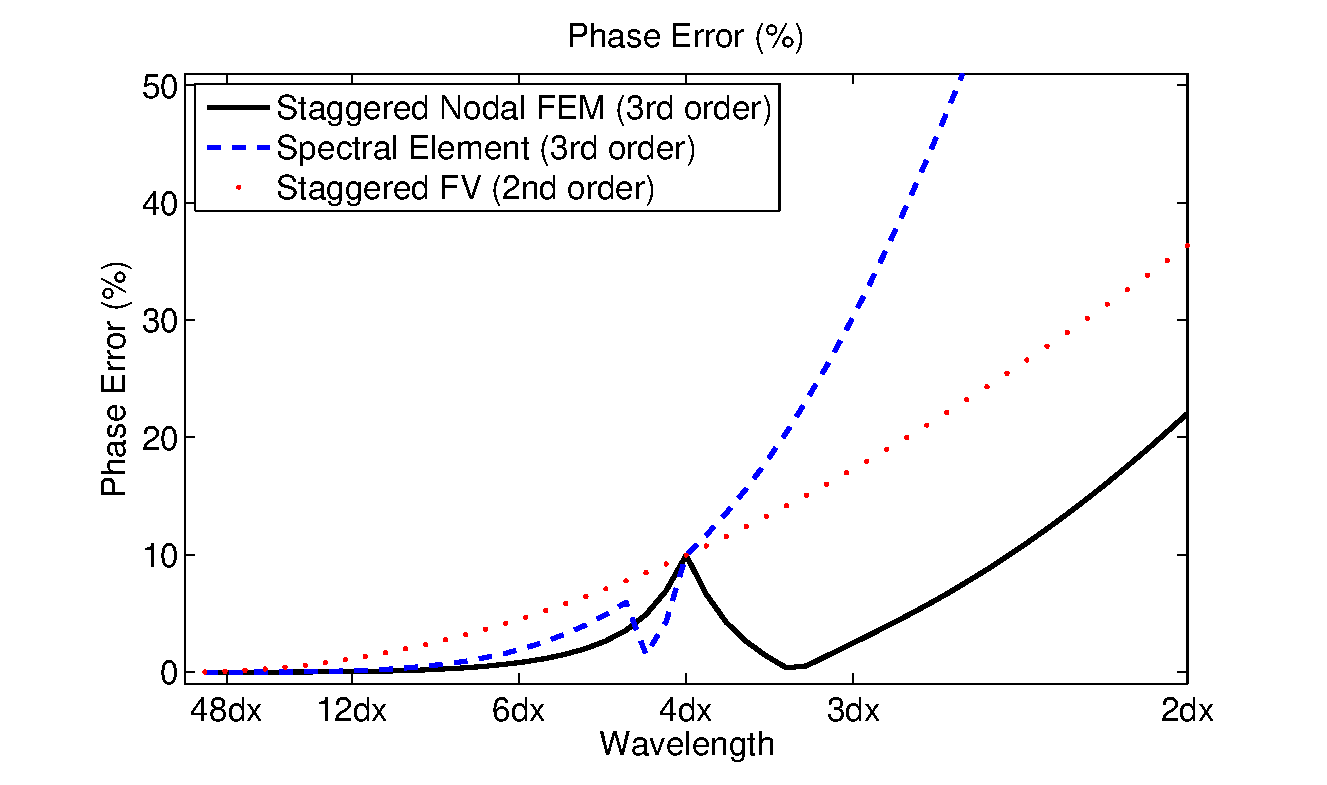
\includegraphics[width=4in, clip=true, trim=0cm 0.1cm 0cm 0.1cm]{PhaseErrors}
\end{center}
\caption{An analysis of phase speed errors of the right-going mode for three non-diffusive discretizations of the 1D wave equation (3rd order SNFEM, 3rd order spectral element and 2nd order staggered FV) as a function of horizontal wavelength.  The unstaggered spectral element method exhibits $100\%$ error for $2 \Delta x$ modes, corresponding to zero phase speed.  Observe that although SNFEM and SE have the same number of degrees of freedom per element, SNFEM boasts the best long-wavelength ($> 4 \Delta x$) and short-wavelength ($< 4 \Delta x$) properties.  The presence of the spectral gap at $4 \Delta x$ will be addressed in this work.} \label{fig:SNFEMEigenstructure}
\end{figure}

\begin{figure}
\begin{center}
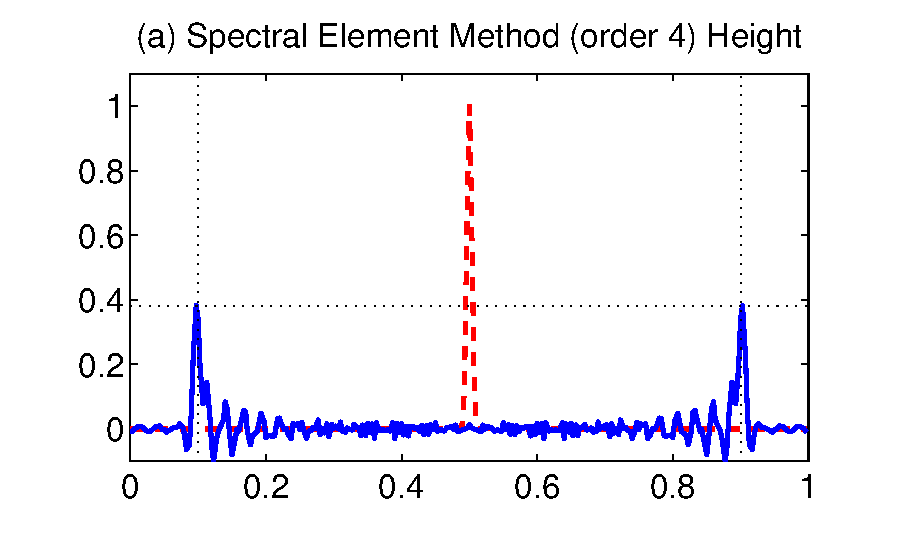
\includegraphics[width=3.2in]{SimulatedBell_SE}
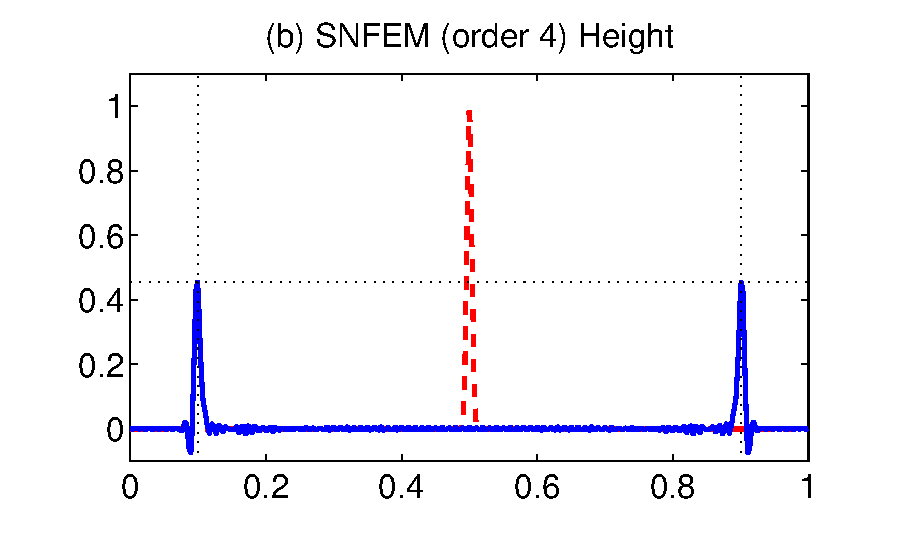
\includegraphics[width=3.2in]{SimulatedBell_SNFEM}
\end{center}
\caption{A sharp Gaussian bell of height $1$ is simulated until $t = 0.4$ under the 1D wave equation using (a) the fourth-order spectral element method and (b) a fourth-order SNFEM formulation.  Initial conditions are shown with red dashed line.  Although both schemes use the same number of degrees of freedom and are energy conservative, the improved phase properties of SNFEM reduce short-wavelength noise in the solution and more closely capture the height of the bell (exact maximum $0.5$).}  \label{fig:SimulatedBell}
\end{figure}

Further, note that since SNFEM are inherently non-diffusive, optimal time step size can be attained using a family of well-known optimal time integrators \cite{kinnmark1984one}.  Several stabilization mechanisms will be studied as part of this proposal, including hyperviscosity \cite{guba2014viscosity, ullrich2014global}, stratification-aware upwinding and a variational multi-scale formulation.

The development of a high-order SNFEM vertical coordinate also has the potential for greatly reducing errors related to pressure gradient errors:  This proposal advocates removing pressure gradient errors by improving the accuracy of the coupling between the horizontal and vertical discrete pressure gradient operators.  Preliminary results suggest that improving the vertical order-of-accuracy from two to four can lead to errors that are about two orders of magnitude smaller.  Errors related to horizontal viscosity will be addressed via the development of a stratification-aware viscous operator.

%\subsubsection{Justification of Hypotheses}

%\textbf{Why are these hypotheses justified?  Why are we using SNFEMs?}

%- Contrast the non-hydrostatic equation set versus traditional approaches using the hydrostatic equations


%The hypotheses of this proposal has been formulated based on past success of massively parallel finite element methods (FEMs) \cite{JDJEKJEONGetal2011IJHPCA}, the analysis of staggered methods performed by \cite{JTTJW2005JCP}, an understanding of the wave-like properties of numerical methods built from \cite{PAUCJ2011JCP}, the analysis of low-order SNFEM performed by \cite{CJCJS2012JCP} and preliminary analysis of SNFEM discussed in section \ref{sec:SNFEM}.  In addition to the central hypothesis stated above, we further hypothesize the following: 

%  This method can be applied in conjunction with the direct stiffness summation operation (which averages co-located state values on GLL nodes) when continuity is desired.  An operator for stabilization / diffusion, which is necessary for the application of these methods to long-term climate simulations, will be developed based on the work of \cite{OGMNLJROMATPAU2013}.  It is well-known that an optimal choice of grid staggering can greatly improve the treatment of atmospheric waves \cite{DAR1994MWR}, but it is not immediately clear how staggering of variables should be handled in the context of FEM.  However, recent efforts by \cite{DBLG2009CS} and \cite{CJCJS2012JCP} have investigated a standard low-order 1D SNFEM staggering and generally found that SNFEM retain the desirable properties of FEM (parallel scalability, mass/energy conservation and a discrete analogue of the gradient, divergence and curl operators).  Further, when the staggering is chosen correctly, these methods also retain the beneficial properties of staggered grid methods.  The PI has also investigated the ability of several standard numerical methods to properly capture the diffusive and dispersive properties of the 1D linear wave equation, and the results suggest that SNFEM greatly outperforms competing methods (see Table \ref{tab:ShortestResolvedWave} and \cite{PAU2013QJRMS}).

%\begin{table}
%\begin{center}
%\begin{tabular}{ccc}
%\hline & \multicolumn{2}{c}{\underline{Shortest Resolved Wave}} \\
%Method & Order 3 & Order 4 \\
%\hline \hline Finite Volume & $12.53\ \Delta x$ & $9.98\ \Delta x$ \\
%Spectral Volume & $11.94\ \Delta x$ & $9.16\ \Delta x$ \\
%Discontinuous Galerkin & $10.01\ \Delta x$ & $7.87\ \Delta x$ \\
%Spectral Element & $8.33\ \Delta x$ & $8.87\ \Delta x$ \\
%SNFEM & $6.68\ \Delta x$ & $5.56\ \Delta x$ \\
%\hline
%\end{tabular}
%\end{center}
%\caption{Shortest wavelength which is resolved to at least 0.5\% error in both the diffusive and dispersive error components, obtained from analysis of the 1D linear wave equation, for several methods of third- and fourth-order accuracy.} \label{tab:ShortestResolvedWave}
%\end{table}

\subsubsection{Static and adaptive mesh refinement} \label{sec:Refinement}

The disparity between global and regional scales makes it difficult to diagnose changes to regional climate that occur due to shifts in the whole Earth system.  Restrictions in software infrastructure and computational cost have inherently limited the finest resolution of our uniform-resolution climate models to 50-100 km, a scale too large to capture many facets of regional climate.  However, the need for regional scale analysis is emphasized in the 2014-29 US CLIVAR Science Plan: ``Adaptation and mitigation decisions in response to climate variability and change are made at a local scale, and a better physical understanding of regional features associated with climate change is essential to garner public support for financial resources that will be required for putting appropriate strategies into action.''  Regional climate modeling, either via dynamical downscaling or variable resolution global models, is necessary to address these needs.

For climate applications, mesh refinement can both improve the resolution of atmospheric flows, and help test physical parameterizations across spatial and temporal scales in a global context, without refining the entire computational domain.  Static mesh refinement techniques offer the opportunity to span global and regional scales and reach the resolutions needed for answering questions relevant to local communities.  Further, adaptive refinement techniques allow for tracking synoptic features that contribute significantly to climate means in the Earth system, such as extra-tropical and tropical cyclones.  These features would benefit from space-time adaptivity to better resolve their fine-scale structure and underlying dynamics.

The adoption of mesh refinement in the global atmospheric modeling community is fairly recent, although a number of major modeling centers are currently pushing this capability to operational general circulation models \cite{skamarock2012mpas, LMHSJL2013MWR, CMZCJMAT2013MWR, mccorquodale2014adaptive}.   Nonetheless, static mesh refinement has been demonstrated to be effective for operational modeling of tropical cyclones \cite{zarzycki2014multidecadal, zarzycki2014using}, large-scale weather systems \cite{rauscher2014impact} and regional climate \cite{rauscher2013exploring, zarzycki2014aquaplanet}.

This proposal will \textbf{build a static and adaptive mesh refinement capability} into the Tempest model using block-structured mesh refinement.

%Similar high-accuracy block-structured adaptive mesh refinement (AMR) approaches have been applied to problems in compressible gas dynamics \cite{mccorquodaleColella:2011, GuzikETAL:2012}.

\subsection{Detail of the Proposed Research} \label{sec:Research}

The goal of this proposal is the development of a next-generation non-hydrostatic atmospheric modeling environment using a horizontally-explicit and vertically-implicit formulation (sec. \ref{sec:UniqueAtmosphere}) that addresses observed problems with terrain-following coordinates (sec. \ref{sec:TopographyPGF}), exhibits optimal scalability on large-scale parallel systems (sec. \ref{sec:FEM}), uses staggering to recover nearly optimal treatment of atmospheric waves (sec. \ref{sec:SNFEM}), and supports static and adaptive mesh refinement (sec. \ref{sec:Refinement}).

%\begin{figure}[t]
%\begin{center}
%\includegraphics[width=6in]{UMJSTest-Results}
%\end{center}
%\caption{A developing non-hydrostatic baroclinic instability simulated in the Tempest framework.  Relative vorticity shown.} \label{fig:TempestBaroclinicInstability}
%\end{figure}

This proposal will use the Tempest framework \cite{ullrich2014global} as a starting point for research tasks T2-T5.  Tempest is a numerical framework (\url{https://github.com/paullric/tempestmodel}) \cite{ullrich2014global} for solving partial differential equations in block-structured geometry implemented in C++ and parallelized using MPI.  The framework has been built by PI Ullrich to improve the ease of experimentation and inter comparison of numerical discretizations, particularly for applications in geophysical fluid dynamics.  The model currently supports a number of (unstaggered) nodal finite-element methods including discontinuous Galerkin (DG) \cite{cockburn2000development}, spectral element (SE) \cite{maday1989spectral} and flux reconstruction (FR) \cite{huynh2007flux}.  Several second-, third- and fourth-order implicit-explicit time integrators (see section \ref{sec:UniqueAtmosphere}) have been implemented for all spatial discretizations.  The model supports both limited-area (Cartesian) domains and global (spherical) domains, via the cubed-sphere grid (see Fig. \ref{fig:CubedSphere}).  Strong scaling tests have been performed on the NERSC Edison supercomputer and optimal scalability up to 24k processor cores was observed.  Work is currently underway to integrate Tempest into the Community Earth System Model \cite{JWHetal2013BAMS} as a next-generation atmospheric dynamical core.

\begin{wrapfigure}[15]{r}{2.2in}
\begin{center}
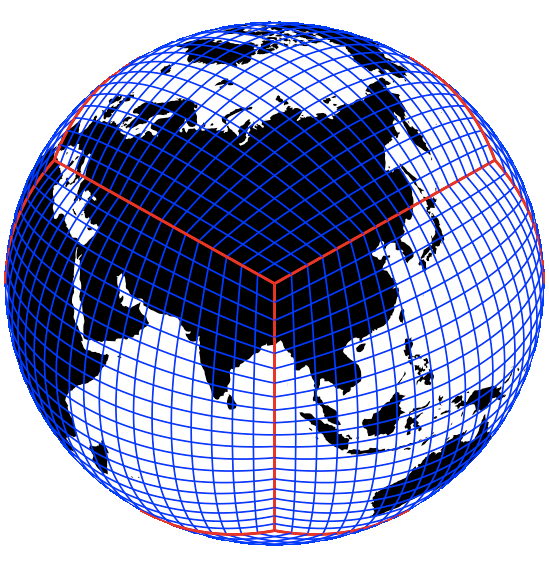
\includegraphics[width=2in]{A_CubedSphere}
\end{center}
\caption{The cubed-sphere grid.} \label{fig:CubedSphere}
\end{wrapfigure}

Once model development is complete, verification must be performed to ensure consistency with analytical test cases, and intercomparison with other dynamical cores.  Recently, a test case suite for 3D atmospheric dynamical cores has been proposed as part of the Dynamical Core Model Intercomparison Project (DCMIP), documented in \cite{DCMIP2012TESTCASES, kent2013dynamical}.  These test suites further provide the opportunity for intercomparison of the SNFEM dynamical core with other operational dynamical cores via DCMIP and other scientific publications.  Once verification is complete, future efforts will tackle the addition of moisture and physical parameterizations to the dynamical core.

The list of research and development tasks to be undertaken for this proposal are described in the following sections.

\subsubsection{(T1) A thorough analysis of 1D and 2D staggered nodal finite element methods} \label{sec:AnalysisSNFEM}

%To a close approximation, the atmosphere is in a state of geostrophic and hydrostatic balance.  The dynamic character of the atmosphere is governed by a slow adjustment process which gives rise to wave motion over all scales.  Accurate treatment of these waves is important to capture departures from geostrophic balance, and to ensure that the adjustment process is correct and free from spurious numerical errors.  As shown by \cite{PHLCJMATRDN2010JAMES}, an accurate treatment of the equations of motion is also important to avoid errors due to grid imprinting.

The capability of a numerical method to capture wave-like motion in atmospheric models is typically evaluated using dispersion analysis.  This mathematical technique decomposes the discrete response in the atmospheric model into diffusive and dispersive errors introduced by the discretization.  Diffusive errors are typically associated with an unphysical loss of wave energy from the system and dispersive errors are associated with unphysical ringing, corresponding to an incorrect treatment of individual wave speeds.  A key paper by \cite{randall1994geostrophic} used dispersion analysis to demonstrate the superior performance of staggered grids for modeling geophysical flows.  More recently, \cite{MAHAW2009SIAMJNA} (and later \cite{melvin2012dispersion}) applied dispersion analysis to the SE method in the context of geophysical motions.  They found that, although the SE method possessed good long-wave characteristics, the unstaggered nature of the scheme led to a short-wavelength regime with unphysical backwards energy propagation.

This proposal will undertake a thorough \textbf{dispersion analysis of SNFEM}, which does not currently exist in the literature.  This analysis will extend preliminary work to 2D geophysical problems and would be incredibly beneficial for determining any outstanding issues with the formulation of the method prior to its use in atmospheric modeling.  In 1D this analysis would need to explore different choices of flux correction function \cite{huynh2007flux} and the resulting impact on accuracy, stability and maximum time step size.  Further, this analysis would examine the effect of modifying the nodal points from GL or GLL nodes.  In 2D this analysis would need to consider all arrangements of nodal values (see Figure \ref{fig:NodalArrangement}).  Based on the results of \cite{randall1994geostrophic} it is hypothesized that the C-grid arrangement of Figure \ref{fig:NodalArrangement}c will produce an optimal dispersion relationship.  Both the linear wave equation and linear shallow water equations (which incorporate Coriolis force) would be analyzed.  This analysis will further address the following questions:

%  Further, this analysis would provide guidance in choosing a SNFEM formulation that preserves desirable geophysical properties, including geostrophic balance on the $f$-plane.  A thorough analysis must address several outstanding questions:

\begin{figure}[t]
\begin{center}
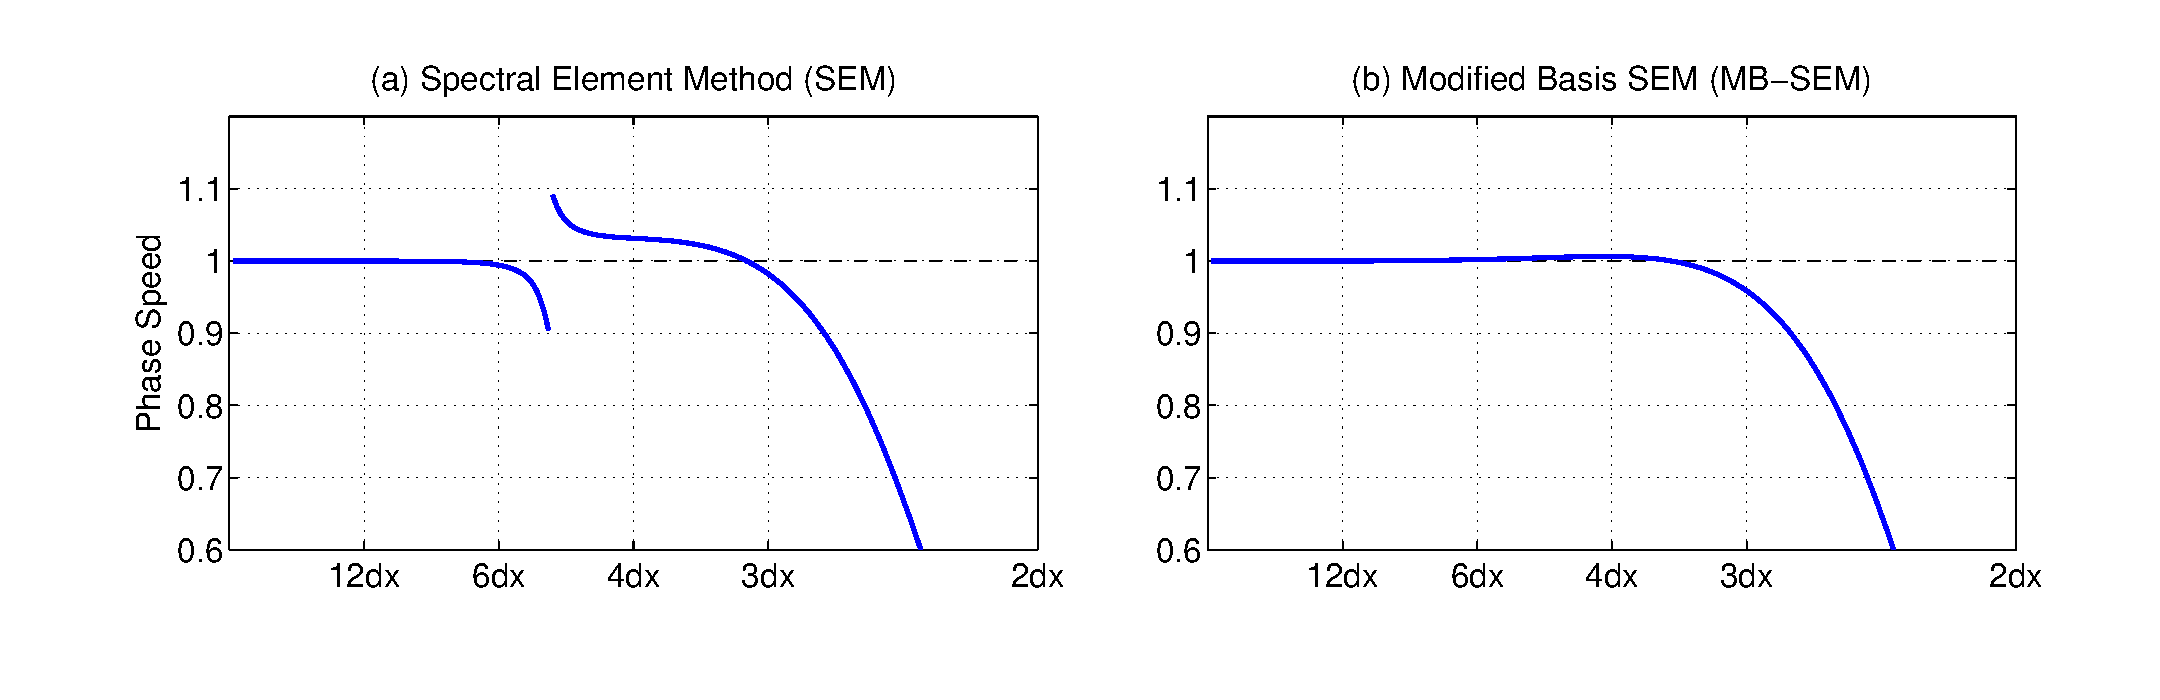
\includegraphics[width=6.5in, clip=true, trim=0cm 1.6cm 0cm 0.7cm]{ModifiedBasisMethod}
\end{center}
\caption{(a) Dispersion relation for the unmodified SE method of order 5 showing a spectral gap and (b) Dispersion relation for the SE method using a modified basis where the spectral gap has been removed.  The horizontal axis gives wavelength in terms of average spacing between nodes $dx$.  The exact phase speed is $c_p = 1$.} \label{fig:SEMDispersionGap}
\end{figure}

\vspace{-0.4cm}
\begin{itemize}
\item \textit{How can SNFEM be configured to avoid the appearance of a spectral gap?}  The ``spectral gap'' is a phenomenon that often appears when an inhomogeneous stencil is used for the spatial discretization (unlike, for example, finite volume methods which use the same stencil for all cells).  It is associated with an unphysical jump in the phase speed (see Figure \ref{fig:SEMDispersionGap}) which can lead to inaccurate treatment of certain wave numbers.  This gap can be fixed by either partial mass lumping \cite{staniforth2013analysis}, the application of dissipation (such as upwinding, as in the discontinuous Galerkin approach), or by an improved choice of the functional space within an element (modified basis method).  The modified basis method has been used by the PI to successfully remove the spectral gap for the SE method and improve the accuracy of the method (see Figure \ref{fig:SEMDispersionGap} and \cite{ullrich2014understanding}).  This project aims to study how the choice of dissipative operator and basis functions affects the spectra of the SNFEM approach, and if the spectral gap can be eliminated for the linear 1D and 2D shallow-water equations using a similar approach.  It is hypothesized that the spectral gap can be completely eliminated at all orders-of-accuracy through a combination of judiciously chosen dissipative operator and/or an improved choice of basis functions.

%\item An extension of the SNFEM analysis to 2D is important to understand the behavior of SNFEM in a context which is relevant to geophysical motions.  In particular, this project is interested in an extension of the 1D analysis to the 2D linear shallow-water equations with non-zero Coriolis parameter $f$.  It is not currently understood if high-order SNFEM will share similar dispersion properties to the staggered finite-difference schemes which were analyzed by \cite{randall1994geostrophic}.  Further, it is known that the arrangement of nodal points can have a significant effect on the dispersive properties of the underlying method.  Consequently, this effort aims to compare and contrast the different arrangements of nodal points (see Figure \ref{fig:NodalArrangement}) and their influence on the wave-capturing properties of the underlying SNFEM.  It is hypothesized that the C-grid arrangement of Figure \ref{fig:NodalArrangement}c will produce an optimal dispersion relationship.

\item \textit{How do SNFEM behave at grid refinement boundaries?}  Atmospheric models that support variable resolution are becoming increasingly important in addressing issues related to extreme weather and regional climate change \cite{skamarock2012mpas}.  However, as pointed out by \cite{ullrich2011analysis}, in the presence of grid refinement staggered grid methods cannot distinguish between incident waves and artificially reflected waves.  As a consequence, energy in the incident mode tends to be reflected at grid refinement interfaces, leading to potential contamination of the solution in a region of enhanced resolution.  This analysis may suggest that grid boundaries may then require nudging or additional dissipation to remove contamination.
\end{itemize}

\vspace{-0.4cm}
\subsubsection{(T2) A SNFEM Vertical Discretization} \label{sec:VerticalSNFEM}

%There has recently been renewed interest in improving the treatment of the vertical discretization in global atmospheric models.  The accurate representation of vertical wave modes is essential for models of the atmosphere, especially for those with wavelengths near the grid scale, where numerical errors typically appear.  Traditionally the vertical coordinate for the non-hydrostatic fluid equations has either been discretized in the Eulerian frame via a second-order Charney-Phillips \cite{JGCNAP1953JAS} or Lorenz grid \cite{AASM1988JAS}, or via a semi-Lagrangian approach such as \cite{SJL2004MWR}.  

The accurate representation of vertical wave modes is essential for models of the atmosphere.  Vertical propagation of energy is essential for major atmospheric phenomena including the Madden-Julien oscillation and quasi-biennial oscillation \cite{madden1971detection, zhang2005madden, baldwin2001quasi}.  Errors in a spatial discretization are often greatly enhanced near the grid scale ($2 \Delta x$) due to the use of an exceptionally large Courant number (see section \ref{sec:UniqueAtmosphere}).  However, little work has been performed to develop high-order vertical coordinates due to a number of outstanding issues.  First, higher-order generalizations must somehow deal with the no-flux boundary conditions at the model bottom and top without loss of accuracy, especially near the surface where accurate treatment of dynamics is paramount.  Second, the choice of vertical coordinate (whether height-based, mass-based or entropy-based) implies an optimal vertical staggering of prognostic variables for maintaining correct behavior for wave motions relevant to the atmosphere \cite{thuburn2005vertical, JT2006QJRMS, MDTRDA2007JCP}.  Third, unstaggered discretizations (that is, discretizations where all prognostic variables are stored on model levels) possess stationary computational modes which can potentially damage the numerical solution and can degrade the quality of the solution.  As in the horizontal direction, unstaggered FEM leads to waves with zero phase speed in the limit as wavelength $\lambda \to 2 \Delta x$ (see Figure \ref{fig:SNFEMEigenstructure}).  Unlike the horizontal, these wave modes can be dramatically enhanced by an implicit treatment of the vertical at high Courant number.

First, we propose to \textbf{develop, analyze and implement the SNFEM machinery for use as an arbitrary-order vertical discretization} for the atmospheric equations of motion, isolating terms which are relevant to vertical motion and solving for these terms implicitly.  The use of SNFEM is natural for vertical discretizations:  No-flux boundary conditions are natural in the context of FEM, and the structure of individual elements (that is, the tendency for nodal values to be concentrated near element edges) lends itself readily to improved resolution in the atmospheric boundary layer.  Further, SNFEM inherits the mimetic properties of SE methods and so the vertical operator will automatically conserve both mass and discrete energy.

Second, we propose to \textbf{understand how acoustic, inertia-gravity waves and the Rossby wave modes} respond to different staggerings of prognostic variables, locations of interior nodes, choice of FR reconstruction function and order-of-accuracy in the context of SNFEM.  This analysis extends the work of \cite{thuburn2005vertical}, which was developed for low-order discretizations.  In total, of the prognostic variables $\rho$, $u$, $v$, $w$ and $\theta$ and the diagnosed mass flux $\mathcal{F}_\rho = \rho w$ and Exner pressure $\Pi$, there are $2^5$ different options for staggering on model levels and interfaces (assuming $\rho$, $u$ and $v$ are kept together).  Of these options only a limited subset exhibit optimal wave-propagation properties and are free of stationary computational modes.

Third, we propose to \textbf{investigate the use of implicit-explicit coupling strategies}, including many from the computational science literature \cite{UASJRRJS1997AMM, CACMHK2003ANM}, for improving horizontal-vertical coupling in the atmospheric model.  Recently, recognizing that high-order coupling is necessary for next-generation non-hydrostatic atmospheric models, many of these methods have been analyzed in an idealized context by \cite{HWSJLNW2013JCP}.


% one approach for obtaining uniform high-order accuracy in both time and space by using a novel strategy for combining the horizontal, vertical and temporal discretization.  The time discretization must account for the treatment of horizontal motions by an explicit discretization and vertical motions by an implicit discretization; a technique known as horizontally explicit vertically implicit (HEVI).  Second-order and higher one-step methods are usually referred to as Implicit-Explicit Runge-Kutta (IMEX-RK) methods, and many such methods have been proposed in the literature \cite{UASJRRJS1997AMM, CACMHK2003ANM}.  Recently, recognizing that high-order coupling is necessary for next-generation non-hydrostatic atmospheric models, many of these methods have been analyzed in the context of HEVI discretizations by \cite{HWSJLNW2013JCP}.

%This proposal aims to generalize and extend the work of \cite{JTTJW2005JCP} to understand how acoustic, inertia-gravity waves and the Rossby wave modes respond to different staggerings of prognostic variables, locations of interior nodes and order-of-accuracy in the context of SNFEM.  

%Other staggering options may be explored in conjunction with the effect of a variable order-of-accuracy.  In addition the following questions will be addressed:

%\begin{table}
%\caption{Composition of interpolation $\mathcal{I}$ and differentiation $\mathcal{D}$ operators for several choices of staggering.  Subscript $e$ denotes variables defined on interfaces (Gauss-Lobatto-Legendre nodes) and $n$ represents variables defined on model levels (Gauss-Lobatto nodes).  For operator $\mathcal{I}$ and $\mathcal{D}$, the subscript denotes the target ($e$ or $n$) and the superscript denotes the origin.  In accordance with \cite{JT2006QJRMS}, the pressure gradient in the vertical is reformulated as $\rho^{-1} \nabla p = \theta \nabla \Pi$, where $\Pi$ is the Exner pressure ($\Pi_n(\rho, \theta) = c_p \left[ R_d \rho \theta / p_0 \right]^{R_d/c_v}$).} \label{tab:StaggeringOperators}

%\begin{center}
%\begin{tabular}{cc|ccc}
%\hline  & & \multicolumn{3}{c}{\underline{Choice of Staggering}} \\
%Variable & Operator & DG $(\rho_n \theta_n u^\xi_n)$ & SNFEM-L $(\rho_n \theta_n, u^\xi_e)$ & SNFEM-CP $(\rho_n, u^\xi_e \theta_e)$ \\
%\hline \hline $\displaystyle \Pi_n$ & & $\Pi_n(\rho_n, \theta_n)$ & $\Pi_n(\rho_n, \theta_n)$ & $\Pi_n(\rho_n, \mathcal{I}_n^e \theta_e)$ \\[2.5ex]
%$\theta$ & $\displaystyle u^\xi \pdiff{\theta}{\xi}$ & $(u^\xi_n) \mathcal{D}_n^n \theta_n$ & $(\mathcal{I}_n^e u^\xi_e) (\mathcal{D}_n^n \theta)$ & $(u^\xi_e) (\mathcal{D}_e^e \theta_e)$ \\[2.5ex]
%$u^\xi$ & $\displaystyle \theta \pdiff{\Pi}{\xi}$ & $\theta_n \mathcal{D}^n_n \Pi_n$ & $(\mathcal{I}_n^e \theta_n) (\mathcal{D}^n_e \Pi_n)$ & $\theta_e (\mathcal{D}^n_e \Pi_n)$ \\[2.5ex]
%$\rho$ & $\displaystyle \frac{1}{J} \pdiff{}{\xi} (J \rho u^\xi)$ & $\displaystyle \frac{1}{J_n} \mathcal{D}^n_n (J_n \rho_n u^\xi_n)$ & $\displaystyle \frac{1}{J_n} \mathcal{D}^e_n \left[ J_e (\mathcal{I}_e^n \rho_n) u^\xi_e \right]$ & $\displaystyle \frac{1}{J_n} \mathcal{D}^e_n \left[ J_e (\mathcal{I}_e^n \rho_n) u^\xi_e \right]$ \\[2.5ex]
%\hline
%\end{tabular}
%\end{center}
%\end{table}

%\begin{itemize}
%\item How do acoustic, inertia-gravity waves and the Rossby wave modes respond to different staggerings of prognostic variables, locations of interior nodes and order-of-accuracy?  This work aims to generalize and extend the work of \cite{JTTJW2005JCP}, who answered this question for the set of second-order central discretizations with arbitrary prognostic variable staggering.  The accurate representation of atmospheric wave modes is essential for models of the atmosphere, especially for the wave modes with the shortest wavelength, where numerical errors typically appear.

%\item What is the optimal approach for solving the implicit system that arises from the vertical discretization?  The matrix system that arises in each column of the model under a SNFEM discretization has a block-tridiagonal structure with a dominant off-diagonal.  This work intends to determine which approach leads to the most efficient solution of the implicit system.  The options for solvers include Jacobian-free Newton-Krylov (JFNK)-type methods, stabilized bi-conjugate gradient methods or a Jacobian construction / direct solver (with or without Schur complement).  Further, this proposal is interested in whether a Rosenbrock approach (that is, only computing a linearly implicit solution to the matrix system such as in \cite{PAUCJ2012MWR}) can be used in place of a fully implicit solution. 
%\end{itemize}

%\subsubsection{Improved Horizontal-Vertical Coupling} \label{sec:CouplingSNFEM}

%This research will investigate one approach for obtaining uniform high-order accuracy in both time and space by using a novel strategy for combining the horizontal, vertical and temporal discretization.  The time discretization must account for the treatment of horizontal motions by an explicit discretization and vertical motions by an implicit discretization; a technique known as horizontally explicit vertically implicit (HEVI).  Second-order and higher one-step methods are usually referred to as Implicit-Explicit Runge-Kutta (IMEX-RK) methods, and many such methods have been proposed in the literature \cite{UASJRRJS1997AMM, CACMHK2003ANM}.  Recently, recognizing that high-order coupling is necessary for next-generation non-hydrostatic atmospheric models, many of these methods have been analyzed in the context of HEVI discretizations by \cite{HWSJLNW2013JCP}.

\subsubsection{(T3) Implementation of SNFEM in the Horizontal} \label{sec:HorizontalSNFEM}

As argued in section \ref{sec:SNFEM}, SNFEM have the potential for greatly improving the treatment of atmospheric waves in atmospheric models.  Following the analysis of (T1) (section \ref{sec:AnalysisSNFEM}), we propose to \textbf{implement SNFEM in the Tempest framework} for operational use in atmospheric modeling.  Overall, we expect that the SNFEM formulation will greatly improve the accuracy of the fluid equation solver and reduce spurious numerical errors which are associated with a poor treatment of waves near the grid scale.  Further, we expect that a high-order horizontal, vertical and implicit-explicit integrator will greatly reduce errors associated with the pressure-gradient problem.

%Once implementation of the horizontal SNFEM has been completed, we will be able to better test its operational performance in the context of increasingly realistic test cases.  In conjunction with the simplified atmospheric model (SAM) physics suite {\color{red}(Ref?)}, we will be able to run tests that include both 3D dry dynamics and moisture and compare with existing atmospheric models.

\subsubsection{(T4) Stabilization of SNFEM}

Although a high-order treatment is expected to partially eliminate pressure gradient errors, linear diffusion of density and pressure along terrain-following surfaces is a major contributor to these errors (see section \ref{sec:TopographyPGF}).  Consequently, we propose \textbf{to develop and test a number of non-linear viscous operators which account for background stratification}.  These techniques are expected to stabilize both FEM and SNFEM formulations without driving anomalous vertical velocity.  The two key techniques we will focus on are stratification-aware upwinding and the variational multiscale method:

\vspace{-0.4cm}
\begin{itemize}
\item Upwinding is a common technique in the context of finite volume and discontinuous Galerkin methods that uses the magnitude of the discontinuity at element edges to drive diffusivity.  For systems of differential equations, upwinding is typically implemented via an approximate Riemann solver applied at element boundaries.  For certain approximate Riemann solvers, such as the local Lax-Friedrichs solver, the effect of upwinding can be characterized as a diffusivity with a coefficient driven by the local wave speed \cite{ullrich2014understanding}.  This proposal will use this observation as a starting point for developing a flow-dependent viscosity that respects local stratification and is further applicable in the context of continuous FEM.

\item The Variational Multiscale (VMS) Method provides stabilization via a physical parameterization of the unresolved sub-grid scales that is added to the original discrete equation. The process begins by reformulating the discrete problem where the prognostic variables are decomposed into a mean/resolved component plus an unknown sub-grid perturbation.  The sub-grid terms are modeled as a function of the parent residual scaled by a local parameter based on the local flow speed and/or the speed of sound. This approach is similar to diffusion like closures used in Large Eddy Simulations and provide a physically based and spatially distributed stabilization that has been shown to be superior to applications of uniform diffusion operators that are typically used in dynamical cores. \cite{hughes1998variational, marras2012variational, marras2013variational}
\end{itemize}

\vspace{-0.4cm}
\subsubsection{(T5) SNFEMs and Block-Based Mesh Refinement}

The final part of this proposal is the development of \textbf{a multi-scale treatment of atmospheric motion using SNFEMs}.  The current formulation of the Tempest model uses an implementation of mesh refinement based on the block-adaptive strategy of \cite{MJBPC1989JCP}, with development in collaboration with the Chombo research group at LBNL \cite{ChomboDesign}.  Since only density and tracers must be conserved (which are discretized with discontinuous flux-based operators), an implementation of SNFEM in the block-based mesh refinement framework will be a fairly straightforward modification of the existing methodology.

\subsection{Research Plan} \label{sec:ResearchPlan}

This project seeks funding for one postdoctoral researcher for two years and one graduate student researcher (GSR) for three years.  Over the course of their employment, the postdoctoral researcher will work with the investigators on the implementation of the SNFEM framework using the Tempest codebase, development of test problems and offer additional assistance with analysis of the SNFEM.  Simultaneously, the graduate student researcher will be in charge of the 1D and 2D analysis of SNFEM, with 2D analysis carrying over into the second year.  In the second year, the graduate student researcher will work to test out the various permutations of SNFEM and study the role of the vertical discretization and coupling mechanism on model accuracy in the presence of steep topography.  Finally, in their third year, the graduate student researcher will be responsible for validation and verification of the 3D SNFEM framework code, including applications to idealized scenarios in atmospheric dynamics.  

Both the postdoctoral research and GSR will benefit from joint advisement by the PI and co-PI.  The proposing institutions are in close geographic proximity, which would allow for frequent travel between locations.  We anticipate meetings will be held between investigators every two weeks via telecommunication, with at least one monthly meeting held in person at either Davis or Berkeley.  Further, the GSR and postdoctoral scholar will have the opportunity to work at Lawrence Berkeley National Laboratory over summer, where both investigators hold faculty scientist positions.

The anticipated schedule for this project is given below:

\begin{tabularx}{\textwidth}{cX}
\hline
\textbf{Year 1} & $\cdot$ 1D analysis of arbitrary-order SNFEM, removal of spectral gap \\
& $\cdot$ 2D linear shallow-water analysis of arbitrary-order SNFEM \\
& $\cdot$ Implementation and testing of SNFEM vertical discretization \\
\hline
\textbf{Year 2} & $\cdot$ Continued analysis of 2D arbitrary-order SNFEM \\
& $\cdot$ Implementation and testing of SNFEM horizontal discretization \\
& $\cdot$ Validation / verification testing of global shallow-water SNFEM code \\
\hline
\textbf{Year 3} & $\cdot$ Analysis of arbitrary-order SNFEM in presence of grid refinement \\
& $\cdot$ Validation / verification testing of 3D Cartesian SNFEM code \\
& $\cdot$ Validation / verification testing of 3D global SNFEM code \\
& $\cdot$ Application of SNFEM framework to idealized atmospheric dynamics experiments \\
\hline
\end{tabularx}

We anticipate that at least five major peer-reviewed publications will arise from this work, including two covering the analysis of SNFEM (for each of the 1D and 2D formulation) and three covering the implementation of the SNFEM framework (for each of the vertical discretization, shallow-water model and 3D multi-resolution global model). Further, this work will be presented at major scientific meetings, including SIAM Geosciences, SIAM Computer Science \& Engineering, the meetings of the American Geophysical Union, the conference for Partial Differential Equations on the Sphere and the Dynamical Core Model Intercomparison Project 2016 Workshop and Summer School.

\subsubsection{Strengths of the Proposal Team}

As emphasized earlier, a key strength of this proposal is the opportunity to build a unique collaboration between computational science and atmospheric science by mutual exchange of expertise.  To this end, both PI Ullrich and co-PI Persson have substantial experience with building interdisciplinary connections between the computational sciences and application areas.  This project will benefit greatly from the PI Ullrich's past experience in atmospheric model development  \cite{PHLRDNPAU2010JCP, PAUCJBVL2010JCP, PHLPAURDN2011SPRINGER, PAUCJ2012MWR, PAUMN2012QJRMS, PAUCJ2012JCP, guba2014viscosity, ullrich2014understanding, ullrich2014global}, numerical analysis \cite{ullrich2011analysis, ullrich2012considerations} and model evaluation \cite{DCMIP2012TESTCASES, ullrich2014proposed, kent2013dynamical, ullrich2014baroclinic}.  It will further benefit from co-PI Persson's work on the development and analysis of DG schemes, including the CDG method \cite{peraire08cdg} and the line-DG method \cite{persson13linedg}), nonlinear stabilization mechanisms \cite{persson06shock}, Large Eddy Simulation \cite{uranga11iles}, and efficient parallel solvers \cite{persson08newtongmres,persson09parallel}, with applications to a range of real-world CFD problems \cite{persson09ale,peraire11dg}.

%\subsection{Implications of the Proposal for Future Applications} \label{sec:FutureWork}

%The work of this proposal has the potential to drive further innovations and form the basis for future research:

%\begin{itemize}
%\item The SNFEM framework that is produced from this work will be used to study dynamical relationships in the tropical atmosphere, following the work of \cite{JABAJM2005JAS,JABAJM2010CMS,JABAJM2012JAS}.  The highly accurate dispersion properties of this method will assist in testing asymptotic relationships governing wave interactions.

%\item The SNFEM framework will be eventually coupled to a stochastic cloud model, following the work of \cite{BKYHJAB2005JAS,BMKJABAJM2010CMS} to study cloud-dynamics interactions and the viability of stochastic cloud models in a global modeling context.

%\item The development of a global SNFEM ocean model will be pursued based on the work of this proposal.  This effort would be beneficial for several reasons:  Staggered grids are ubiquitous in the global ocean modeling community.  Consequently, the adoption of SNFEM for ocean modeling would be able to leverage existing technologies, while improving the spatial accuracy of existing methods.  This approach would also have similar near-optimal dispersive properties as SNFEM for the atmosphere.  This work could quickly lead to the use of a coupled atmosphere-ocean model based on SNFEM that would preserve numerical consistency between the atmosphere and ocean model component.
%\end{itemize}

\subsubsection{Prior NSF Support}

Co-PI Persson has previously been supported by NSF through grant CMMI-0928785,
High Performance Simulation Tools for Complex MEMS Resonator Design,
09/01/2009-08/31/2013, \$360,775. In this work, a new time-dependent DG
formulation for elastodynamics based on the Compact DG method was
developed. This scheme was used for a number of investigations of
micro-mechanical resonators, for example confirming phenomena observed by
experiments regarding the strong dependency of the quality factors on the film
thickness. A new DG PML formulation was also developed, extending it to a
variety of curvilinear coordinate systems with applications to a number of
technologically relevant problem classes, and a framework for using error maps
for selection of optimal PML parameters.  The project funded a Ph.D. student,
Dr. Koki Sagiyama, in his Ph.D. thesis \cite{sagiyama13thesis}. The major
publications that Co-PI Persson was co-authoring as part of this project are
\cite{govindjee12resonator} and \cite{sagiyama14pml}.

%\clearpage
%\bibliography{HybridFiniteElements}
\bibliographystyle{siam}
{\setbox0\vbox{\bibliography{StaggeredFiniteElements}}}

\end{document}
